\chapter{The Steve Tutorial} \label{ch:tutorial}

% It might be worthwhile to divide this into three major sections:
%
% 1. General purpose computing
% 2. Packet specification
% 3. Pipeline specification
%    - decoders
%    - flow tables

The primary focus of the Steve Programming Language is to provide features for
defining and connecting the pipeline processing stages described in Chapter
\ref{ch:pipeline_model}. This chapter will explain how a user writes each of these
components. Specifically, this chapter will discuss how headers are represented, how to
write decoders, how to write tables, and how to apply actions to packets.

At the end of this chapter, four network applications will be presented in Section \ref{tut:examples}: a simple MAC
learning switch, an IPv4 learning switch, a stateless TCP/UDP firewall, and a wire. Many of the examples
presented throughout this chapter are just smaller parts of these applications
presented in isolation. This tutorial will slowly build
up these little components and explain what they do before finally presenting
the complete program at the end.

Semantics and limitations of Steve will be mentioned throughout this chapter, 
but only in minor detail. For the complete semantic description of
Steve, including grammar, typing rules, and other restrictions, see the Reference Guide in Chapter \ref{ch:users_guide}.

\section{General Purpose Language Features} \label{tut:gen_purp}

Steve supports language features that can be considered
\textit{general purpose}. They are common to most programming
languages and are not explicitly for packet processing, though they may prove
useful.

\subsection{Literals} \label{tut:literal}

Steve supports decimal, binary, and hexadecimal integer literals. Steve does not
currently support things like IP address literals or MAC address literals.

Hexadecimal literals all start with the prefix \texttt{0x} followed by any
number of digits between \texttt{0} and \texttt{9}. Binary literals all start with the prefix \texttt{0b} followed by any number of
\texttt{0}'s and \texttt{1}'s.

These integer literals can be written as follows.

\begin{codepage}
\begin{lstlisting}
17 // Decimal literal
0x11 // Hexadecimal 17
0x00010001 // Binary 17
\end{lstlisting}
\end{codepage}
 
The underscore (\texttt{\_}) can optionally be used as a digit separator (like 
Java) for hexadecimal and binary literals with no impact on the value of that 
literal.
This is purely for organization and readability.

\begin{codepage}
\begin{lstlisting}
0b10101010
0b1010_1010

0x0800
0x08_00
\end{lstlisting}
\end{codepage}

Steve also supports character and string literals which are useful for
logging through functions (described in Section \ref{tut:function}).
For example:

\begin{codepage}
\begin{lstlisting}
'H' // A character.
"Hello, World." // A string literal.
\end{lstlisting}
\end{codepage}

\subsection{Variables} \label{tut:variable}

Steve allows for the allocation of both local and global variables. 
A variable named \texttt{x} which holds an integer \texttt{10} is written
as follows. 

\begin{codepage}
\begin{lstlisting}
var x : int = 10;
\end{lstlisting}
\end{codepage}

The type of the variable, \texttt{int}, follows the colon
(\texttt{:}). New values can be assigned to variables like so.

\begin{codepage}
\begin{lstlisting}
x = 1;
\end{lstlisting}
\end{codepage}

The range of common arithmetic and bitwise operations are also supported. The 
complete set of arithmetic and bitwise operations can be found in Section
\ref{guide:binary_expr}.

\begin{codepage}
\begin{lstlisting}
var y : int = 2;
var z : int = 3;
y = x + y; // Addition
z = z << 4; // Left shift
var w : int = y & z; // Bitwise And
\end{lstlisting}
\end{codepage}

\subsection{Conditional Statements} \label{tut:condition}

Steve supports two conditional statements for decision making: the \texttt{if} statement and the \texttt{match} statement. The \texttt{if} statement is the same as most C-like languages.

\begin{codepage}
\begin{lstlisting}
var a : bool = true;
var b : bool = false;
if (a || b) { }
if (a && b) { ... }
else if (a) { ... }
else { ... }
\end{lstlisting}
\end{codepage}

A \texttt{match} statement allows for a decision to be made given a number of 
possible case values. 
This is similar to a C-like switch statement, with the only
major difference being that there is no \textit{fall-through} behavior. In other
words, after the execution of a \texttt{case} statement, control jumps out of the 
\texttt{match} statement rather than moving to the next case (i.e. an implied 
\texttt{break}). 
The condition and labels must be integers just like in C. 
A \texttt{match} statement can be written as follows.

\begin{codepage}
\begin{lstlisting}
match (x) {
  case 0: x = x + 1;
  // Multiple statements following the label must be
  // enclosed in a block.
  case 1: {
    x = x + 2;
    y = y * x;
  }
  // The default case statement.
  miss: x = 0;
}
\end{lstlisting}
\end{codepage}

Here, if \texttt{x} equals \texttt{0}, then \texttt{x = x + 1} gets executed. If
\texttt{x} equals \texttt{1}, then two statements get executed in order:
\texttt{x = x + 2}, then \texttt{y = y * x}. If \texttt{x} is neither, then
\texttt{x = 0} is executed.

\subsection{While Loops} \label{tut:while}

The \texttt{while} loop in Steve is the same as C-like languages. 
They also support the \texttt{break} and \texttt{continue} statements for limited
branching abilities inside a loop. The following is a basic \texttt{while} loop in Steve.

\begin{codepage}
\begin{lstlisting}
var x : int = 0;
var z : int = 0;
while (x < 5) {
  x = x + 1;
  if (x == 3)
    continue;
  if (z == 2)
    break;
  z = z + 1;
}
\end{lstlisting}
\end{codepage}

The usage of \texttt{while} loops in packet processing right now is rather limited. Usage
of loops will rarely come up in defining pipeline processing stages. However,
they may become more useful as other features are added.

\subsection{Functions} \label{tut:function}

Steve supports writing simple functions, though the syntax is a little different
from C-like languages.
A function named \texttt{sum} which takes two
integers, \texttt{a} and \texttt{b}, and returned their sum is written as follows.

\begin{codepage}
\begin{lstlisting}
def sum(a : int, b : int) -> int {
  return a + b;
}
\end{lstlisting}
\end{codepage}

The return type follows the \texttt{->} in Steve functions. To call
the \texttt{sum} function one would write the following. The result of the call to
\texttt{sum(x,y)} would be \texttt{3}.

\begin{codepage}
\begin{lstlisting}
var x : int = 1;
var y : int = 2;
var z : int = sum(x, y);
\end{lstlisting}
\end{codepage}

\subsection{Foreign Functions} \label{tut:foreign}

By default, all Steve compiled applications are linked against the C runtime
library. Steve applications may also be linked against other libraries.
Steve programmers may call functions in linked libraries by first declaring
them in the Steve application using a \emph{foreign function} with the same
function signature.

\begin{codepage}
\begin{lstlisting}
foreign def puts(input : char[]) -> int;
// ...
puts("Hello, World.");
\end{lstlisting}
\end{codepage}

Here, this foreign function links to the C standard \texttt{puts} function
for text output. It may be called like any other function.

\section{Layouts} \label{tut:layout}

A \textit{layout} is used to describe 
the \textit{structure} of a packet header.
More specifically, they describe \textit{what} fields are present, their
\textit{lengths}, the \textit{order} in which they appear, and their
\textit{relative offset} from the beginning of the header. 
Decoders use layout information to reason about extracting fields.

%A layout and a header are two different concepts.
%It is important to make this distinction clear. A layout is like a blueprint for
%a header. It gives us information; it \textit{describes} that header. The header
%is an actual sequence of bits, a portion of the packet, which is taken off of the
%network. The header \textit{exists} whereas a layout helps the Steve application
%\textit{understand} it.

A \emph{layout declaration} (\ref{guide:layout}) is used to write a layout.
The simplest example to begin with is the Ethernet frame header \cite{eth_std}.
The corresponding layout would look like the following.  

\begin{codepage}
\begin{lstlisting}
layout ethernet {
	dst  : uint(48); // 48 bits.
	src  : uint(48); // 48 bits.
	type : uint(16); // 16 bits.
}
\end{lstlisting}
\end{codepage}

Every layout has a name (\texttt{ethernet}) and a sequence of field declarations
which describe the fields contained within the header.
This ethernet layout has three such field declarations (\texttt{dst}, \texttt{src},
and \texttt{type}).
Each field declaration has a name and a type that describes valid operations and
value ranges for that field.
To reduce errors related to working with byte buffers, Steve allows header fields to
be represented as arbitrary-precision, signed or unsigned, integer types.
The precision denotes the length of the field in bits.
Here, \texttt{dst} and \texttt{src} fields are 48 bits long and \texttt{type} is
16 bits long.

The \textit{relative offset} of each field is the number of bits it is away
from the beginning of the header. The first field will always have a relative
offset of 0 bits. The relative offset of each subsequent field is equal to the
sum of the lengths of all fields preceding it. Here, \texttt{dst} has a relative
offset of 0 bits, \texttt{src} has one of 48 bits (6 bytes), and \texttt{type} has one of
96 bits (12 bytes).

The field declarations must appear in the order with which they would normally appear
in an ethernet header. Field ordering should always be
preserved when declaring layouts. If the ordering is incorrect, decoders will
assume a sequence of bits is a certain field when it truly is not. 

Not all header structures are as simple as the ethernet header. Sometimes one
must deal with headers nested inside headers. Steve supports nested layouts
to describe this nested header structures.
The following presents such a case where the programmer expects a VLAN header
\cite{vlan_std} nested before the \texttt{type} field of an ethernet
header.

\begin{codepage}
\begin{lstlisting}
// Layouts may be nested like this.
layout ethernet {
  dst  : uint(48);
  src  : uint(48);
  vtag : vlan; // Nested layout
  type : uint(16);
}

layout vlan {
  ethertype : uint(16);
  tci : uint(16);
}
\end{lstlisting}
\end{codepage}

In this example, two layouts are declared: \texttt{ethernet} and \texttt{vlan}. To
achieve a nested layout a field named \texttt{vtag} is added to
\texttt{ethernet} and its type is given as the name of another layout (
\texttt{vlan}). The length of the \texttt{vtag} field would be the sum of
its fields, in this case, 32 bits (4 bytes).

With the way
layouts are described and written, it is easy to draw the comparison between 
layouts and
class types (or record types). \textit{Layouts are not the same concept as 
classes.} Layouts are much stricter.

First, \textit{the types of fields are restricted}. Fields may only
have two types: integer (\ref{guide:integer_type}) and layout
(\ref{guide:layout_type}). There may be varying kinds of integer (e.g.
precisions, signed, unsigned, etc.), but the precision of each integer must also
be \textit{byte-aligned}, that is, a multiple of 8.

Second, the most important distinction is that \textit{objects of layout type
can never be created}. Layouts may not appear as the type of parameters, nor may
they appear as return types. All of the following are considered ill-formed.

\begin{codepage}
\begin{lstlisting}
layout L1 { f1 : uint; f2 : uint(16); }
var x : L1 = 0;
def foo(y : L1) -> L1 { ... }
\end{lstlisting}
\end{codepage}

Layouts are distinct from the headers that they describe.
The sole purpose of layouts is to allow decoders to reason about the logical 
structure of a header in memory.
The memory for packets and their headers exist independent of a running Steve 
application.
To create an object of layout type would imply the need to create new headers,
which is not currently supported by Steve.

%Additionally, there are a number
%of concerns related to constructing objects of layout type, thus such behavior
%is not allowed. For further details on layout limitations, refer to Section
%\ref{guide:no_dst} in the Reference Guide.

Another important thing to note is that Steve does not currently support dynamically
sized types (DST). A DST is a type whose size is predicated upon some value
known only during runtime. These DST's are used to represent fields whose
lengths are dynamic. Some examples of dynamic length fields are the
\texttt{options} fields in IPv4, IPv6 extended, and TCP headers \cite{ipv4_std, ipv6_std,
tcp_std}.

DST's are a language feature that will eventually be added, but are outside the
current implementation. Because of this, fields whose lengths are dynamic cannot
currently be declared, extracted, nor used. The existence and eventual support
of DST's is one of the reasons why objects of layout type cannot be created.
This is further discussed in Section \ref{guide:no_dst}.

The following example presents a case where some of these limitations become relevant -- the IPv4 layout.

\begin{codepage}
\begin{lstlisting}
layout ipv4 {
  version_ihl : uint(8); // Non-byte aligned fields are merged.
  dscp_ecn    : uint(8); // This is merged, too.
  len         : uint(16);
  id          : uint(16);
  fragment    : uint(16); // Fragment flags and offset merged.
  ttl         : uint(8);
  protocol    : uint(8);
  checksum    : uint(16);
  src         : uint(32);
  dst         : uint(32);
  // Options field omitted because it is a DST.
}
\end{lstlisting}
\end{codepage}

In this example, \texttt{version} (a 4 bit field) has to be
merged with \texttt{ihl} (internet header length) (also a 4 bit field) to
achieve byte alignment. The same is true for \texttt{dscp} and \texttt{ecn}. The
\texttt{fragment} field, typically composed of three 1 bit flags and a 13 bit
fragment offset field, is merged into a single 16 bit field. 
Bitwise-And and bit shifting is needed to recover the needed bits.
Examples will come up later when an IPv4 decoder is discussed in
Sections \ref{tut:decoder_access} and \ref{tut:learning_router}.

\section{Decoders} \label{tut:decoder}

Decoders are special purpose functions
used to extract fields from a single header. 
They implicitly take context data structures as arguments and 
operate on them.
A decoder conforms to a layout specification.
Layout information allows the decoder to determine where fields
are located in a header and how long they are.


%\begin{itemize}
%\item Which header is being decoded?
%
%\item What fields from the header are needed and why?
%
%\item How will these fields be used? Will they be used in arithmetic or 
%
%\item \textit{Actions} (described later in Section \ref{tut:action}) are used to manipulate packet fields, forward packets,
%and add/remove flow entries from tables. What actions must be be taken on the packet?
%
%\item Where must the packet be sent next? Must it be further decoded or can it be sent to table matching for decision making?
%\end{itemize}

\subsection{The Basic Decoder Form} \label{tut:basic_decoder}

A decoder is written using a \textit{decoder declaration} (\ref{guide:decoder}).
The most common decoder written is likely the ethernet decoder. The following
is the basic form of an ethernet decoder.

\begin{codepage}
\begin{lstlisting}
decoder start eth_d(ethernet) { ... }
\end{lstlisting}
\end{codepage}

A decoder declaration has four important parts: 
1) a name (\texttt{eth\_d}), 
2) a \textit{layout rule} (\texttt{ethernet}),
3) a body, and
4) the (optional) \texttt{start} keyword.

The decoding process conforms to the layout rule and uses it to reason
about the location and lengths of fields within the header it is decoding.
Decoder operations are placed in the body delimited by $\lbrace\rbrace$.
The \texttt{start} keyword identifies this decoder as the \emph{starting
decoder}. 

A starting decoder is the root of the pipeline.
By extension there can only be one starting decoder.
Every packet must be processed by the starting decoder first.
Since Ethernet is the most common Layer 2 framing protocol, it will
likely be the root of almost all pipelines.

\subsection{Extractions} \label{tut:decoder_extract}

An \textit{extract declaration} (\ref{guide:extract}) in the decoder's body
instructs it to extract the given field. Extracted fields, or extractions,
for short, may then be used by the program as a variable.
The following example expands the body of the \texttt{eth\_d} decoder 
with extract declarations.

\begin{codepage}
\begin{lstlisting}
decoder start eth_d(ethernet) {
	extract ethernet.dst;
	extract ethernet.type;
	// ...
}
\end{lstlisting}
\end{codepage}

Each extract declaration gives a \emph{field name} (\ref{guide:field_name}) 
which tells the decoder which field is being extracted. 
In this example, there are
two such extract declarations which instruct the decoder to extract
the fields \texttt{ethernet.dst} and \texttt{ethernet.type}.
The compiler generates \textit{(offset, length)} pairs 
denoting the relative offset and length of the field
from the field names and layout rule. 
The programmer is never burdened with the process of manually specifying
which bytes form a field.

Only field names which refer to fields in the layout rule may be used. For example, it would not be possible to extract \texttt{ipv4.protocol} in the \texttt{eth\_d} decoder. 
It obviously make no sense to extract a field not in the header. 

\subsection{How Decoder's Extract Fields} \label{tut:extract_how}

The Steve language ensures that decoders have constrained
access to a subset of contiguous bytes in a packet buffer.
This is known as its \emph{view} of the packet.

A decoder's view begins where the header it decodes begins, and ends
(implicitly) where that header ends. 
This constrained region is enforced by the definition of its layout rule. 
That is, a decoder only knows about bytes up to (and including the final field in
its layout rule and cannot know about or access any fields past that point.

A packet's context maintains the beginning of the current view using
a \emph{view index}. Once a decoder is finished executing, it is
responsible for shifting this view index so that it refers to the
first byte of the next header.

Figure \ref{fg:decoding} demonstrates how decoders extract fields and
how this view mechanism is applied on an actual packet instance. 
Here, the Steve application decodes a typical packet 
containing ethernet, IPv4, and TCP headers.

\begin{figure}[ht]
\begin{subfigure}[t, scale=0.5]{.45\textwidth}
  \centering
  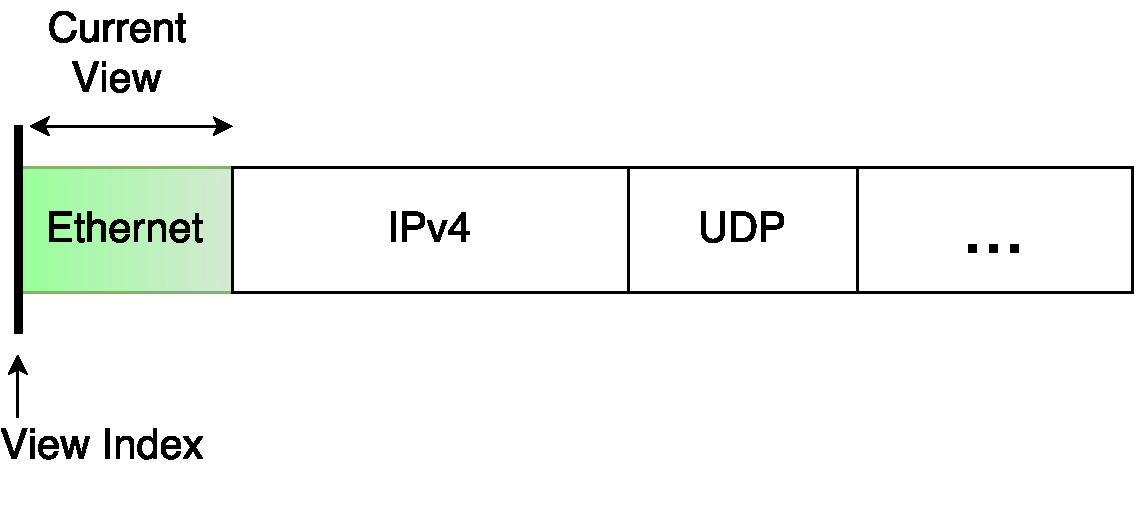
\includegraphics[width=\linewidth]{view1}
  \caption{The view of the starting decoder, in this case, the ethernet
decoder. The beginning of the view is the beginning of the ethernet
header, which is also the beginning of the packet.}
  \label{fg:view1}
\end{subfigure}%
\hfill
\begin{subfigure}[t, scale=0.5]{0.45\textwidth}
  \centering
  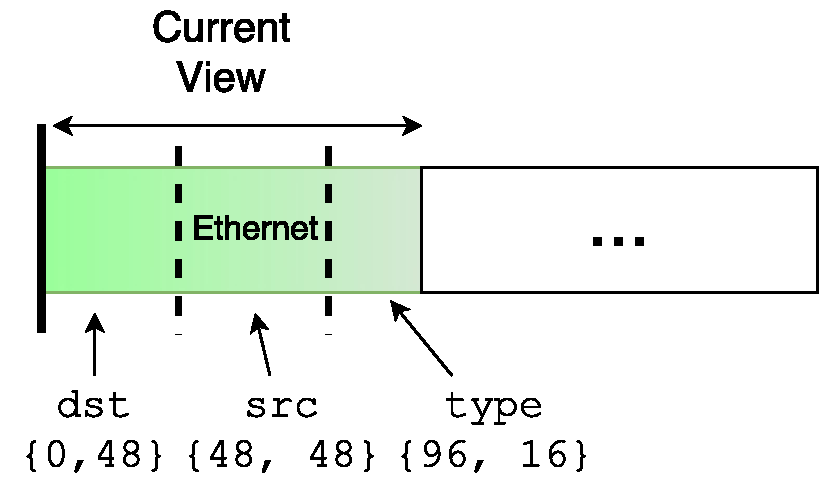
\includegraphics[width=.8\linewidth]{view2}
  \caption{The beginning of a field is discovered by its relative offset from
the beginning of the view. The end is determined by the field's length. The
field \texttt{dst} is 0 bytes from the beginning, \texttt{src} is 6 bytes in,
and \texttt{type} is 12 bytes in.}
  \label{fg:view2}
\end{subfigure}

\begin{subfigure}[t]{.45\textwidth}
  \centering
  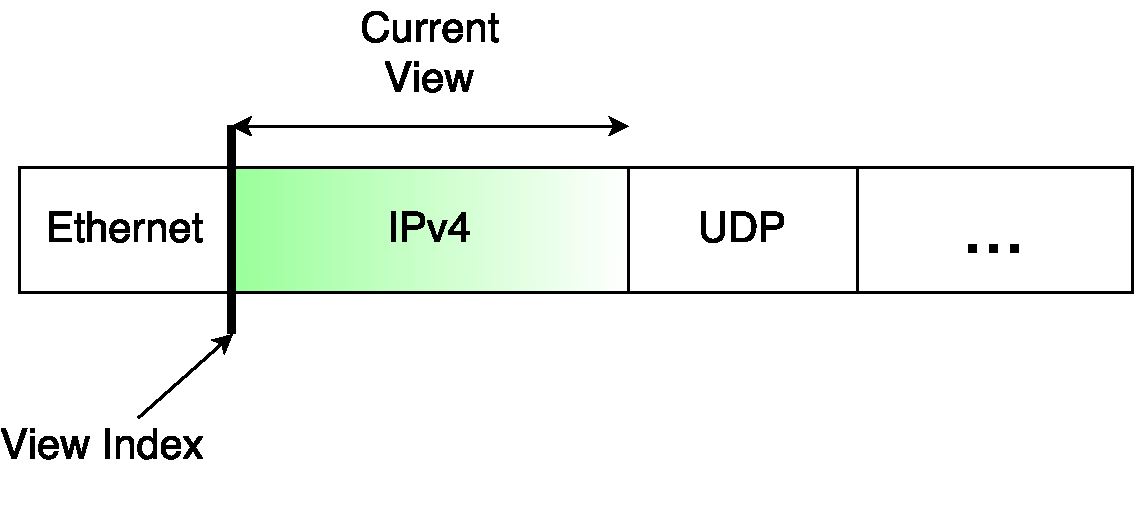
\includegraphics[width=\linewidth]{view3}
  \caption{When a decoder is finished working, it \textit{shifts} the view to
the next header. The shift moves the beginning of the view by the length of the
header -- 14 bytes.}
  \label{fg:view3}
\end{subfigure}%
\caption{A demonstration of the decoding process in action.}
\label{fg:decoding}
\end{figure}

 
The view index always starts at the beginning of the packet.
In Figure \ref{fg:view1}, the first header is ethernet.
In Figure \ref{fg:view2}, the three fields of the ethernet header
are extracted.

When the compiler generates \textit{(offset, length)} pairs,
the offset value is relative to the view index. That is, the
absolute offset of the field in the packet is the view index plus 
the relative offset in the pair.
The absolute offset and length are saved in the context binding environment.
In Figure \ref{fg:view2}, the pairs \textit{(0, 48)} (\texttt{ethernet.dst}),
\textit{(48, 48)} (\texttt{ethernet.src}), and \textit{(96, 16)} 
(\texttt{ethernet.type}) are stored in the context.

%Each field in the header is discovered by information gathered by the layout
%rule. The layout rule tells a decoder the location, or relative offset, of
%each field from the beginning of the header (which is equivalent to the
%beginning of the view). It also gives the length of each
%field. From here, a decoder can go about discovering which bits form each
%field as demonstrated in Figure \ref{fg:view2}.

When a decoder finishes, it \textit{shifts} the view index, as seen in Figure
\ref{fg:view3}. The beginning of the view is moved by the length of header.
The view now starts one byte \textit{after} the previous header's final byte. 
All decoders are responsible for shifting the view in
preparation for the next decoder. Once the next decoder is reached, its view is
already on the header it decodes.

This process continues until all decoders are finished.
If at any point a layout is silently ill-defined 
(longer than the remaining packet memory), and a decoder tries
to extract a field which is past the bounds of the packet, the packet
is immediately dropped before the extraction completes.

\subsection{Accessing Extracted Fields} \label{tut:decoder_access}


Once a field has been extracted, getting its value is similar to using
it as variable.
To get the value of an extraction
the \textit{field access expression} (\ref{guide:field_access_expr}) is used.
A field access expression is essentially a field name being used where
an expression is expected. This is similar to using a variable name
in an expression to represent the value of the variable.

The following example demonstrates how the value of the \texttt{ethernet.type} 
extraction might be used.

\begin{codepage}
\begin{lstlisting}
decoder start eth_d(ethernet) {
  extract ethernet.dst;
  extract ethernet.type;
  if (ethernet.type >= 0x600) {
    // The type determines what header comes next...
  }
  else if (ethernet.type <= 0x05dc) {
    // The type is the length of the entire packet...
  }
}
\end{lstlisting}
\end{codepage}

A typical operation on an ethernet header is determining which protocol
it encapsulates, i.e. the header which comes next. This is indicated
by the value stored in \texttt{ethernet.type}.
The IEEE ethernet standard says that \texttt{ethernet.type} fields greater than 
or equal to \texttt{0x600} indicate the next header's protocol \cite{eth_std}. 
Any \texttt{type} fields less than \texttt{0x05dc} indicate the ethernet frame's 
length. 
Here, field access is used to compare \texttt{ethernet.type} to 
hexadecimal literals in an \texttt{if-else} statement to determine the meaning of 
that field.

Extraction values can also be used in arithmetic operations, comparison 
operations, bitwise operations, function calls,
and can be stored and assigned to variables. The following example presents
a trivial IPv4 decoder demonstrating some of these basic operations.

\begin{codepage}
\begin{lstlisting}
decoder ipv4_d(ipv4) {
  extract ipv4.version_ihl; // Use this to get header length.
  extract ipv4.dscp_ecn;
  extract ipv4.len;
  extract ipv4.id;
  extract ipv4.fragment;
  extract ipv4.ttl;
  extract ipv4.protocol;
  extract ipv4.checksum;
  extract ipv4.src;
  extract ipv4.dst;

  var pktlen : uint = ipv4.len; // Variable assignment
  var ihl : uint(8) = ipv4.version_ihl & 0x0f; // Bitwise AND
  var version : uint(8) = ipv4.version_ihl >> 4; // Right shift
  // ...
}
\end{lstlisting}
\end{codepage}

This example presents a solution for recovering non-byte aligned
fields. A bitwise-AND (\ref{guide:bitwise_expr}) is used on \texttt{ipv4.version\_ihl}
with \texttt{0x0f} to recover the \texttt{ihl} field. The 
\texttt{ipv4.version\_ihl} is left-shift by 4 bits to get the \texttt{version} field.

Extractions can be passed to functions as well. A convenient use case is 
calculating the checksum for the IPv4 header. 
The following example extends the IPv4 decoder with a few more operations.

\begin{codepage}
\begin{lstlisting}
decoder ipv4_d(ipv4) {
  // ...
  
  // Calculate a checksum by calling a function.
  var checksum : uint(16) =
      ipv4_checksum(ipv4.version_ihl, ipv4.dscp_ecn, ipv4.len, 
                    ipv4.id, ipv4.fragment, ipv4.ttl, 
                    ipv4.protocol, ipv4.src, ipv4.dst);

  // Check the checksum against the header's checksum.
  if (checksum != ipv4.checksum)
	  drop;
  // Drop time-to-live expired packets.
  if (ipv4.ttl == 0)
    drop;

  set ipv4.ttl = ipv4.ttl - 1; // Decrement time-to-live
  // The ttl has changed, so a new checksum must be calculated.
  set ipv4.checksum =
    ipv4_checksum(ipv4.version_ihl, ipv4.dscp_ecn, ipv4.len, 
                  ipv4.id, ipv4.fragment, ipv4.ttl, 
                  ipv4.protocol, ipv4.src, ipv4.dst);
}
\end{lstlisting}
\end{codepage}

Fields from the IPv4 header are passed to a function named 
\texttt{ipv4\_checksum} (whose definition has been elided for brevity). The 
resulting checksum is compared against the current checksum using an \texttt{if} 
statement. If they do not compare equal, then the packet is dropped using the 
\texttt{drop} action.

Decrementing the time-to-live (\texttt{ipv4.ttl}) is another common operation. 
First the time-to-live is checked to see if it is \texttt{0}. If it is, then the 
packet's lifetime has expired and it will be dropped. If the packet is still 
valid, the field is decremented using simple subtraction and is set using the 
\texttt{set} action. Because a field has been changed in the IPv4 
header, the checksum must be recalculated and set with the new checksum.

Field access expressions do have a number of limitations. The following example
demonstrates some of them.

\begin{codepage}
\begin{lstlisting}
decoder start eth_d(ethernet) {
  // Error: Cannot use eth.type before its extracted.
  if (ethernet.type >= 0x600) { }
  extract ethernet.type;
  // Error: Cannot assign to a field this way.
  ethernet.type = 0x800;
  // OK: A set action must be used instead.
  set ethernet.type = 0x800;
}

decoder ipv4_decode(ipv4) {
  // Error: This decoder does not decode ethernet.
  extract ethernet.type;
  // Error: ethernet.type was not extracted by this decoder.
  if (ethernet.type == 0x800) { }
}
\end{lstlisting}
\end{codepage}

A field access expression can only be used \textit{after} an extract declaration
is made for that field since it is impossible to recover the value of a
field which has not been extracted. By extensions, they cannot be used in
decoders which have not extracted that field. A decoder focuses on exactly one
header and has no knowledge of previous headers or extractions.

Field access expressions cannot be assigned to like a variable. To modify the
value of a field, a \texttt{set} action must be used instead.

\subsection{Moving to Other Stages} \label{tut:decoder_next}

Once the current stage has finished its work, the programmer may decide
to send the packet to another pipeline stage.
Chapter \ref{ch:pipeline_model} describes that decoding and
table matching stages can be chained together in a number of flexible ways.
Any stage may move a packet to a new decoder or a new table.

To move to another decoding stage, the \texttt{decode} action (\ref{guide:decode_action})
is used. The following example bridges the ethernet and IPv4 decoders
declared in earlier examples. Extract declarations are elided for
brevity.

\begin{codepage}
\begin{lstlisting}
decoder start eth_d(ethernet) {
	// ...
	if (ethernet.type >= 0x600)
	    match (ethernet.type) {
	      case 0x800: decode ipv4_d;
	    }
}

decoder ipv4_d(ipv4) { ... }
\end{lstlisting}
\end{codepage}

The \texttt{match} statement is used to check if \texttt{ethernet.type} is equal to
\texttt{0x800}. If it is, then it confirms the next header is IPv4 and the \texttt{decode} action moves the packet to the IPv4 decoder.

To transition to a table matching stage, a \texttt{goto} action (\ref{guide:goto}) (not
to be confused with a C-like \texttt{goto}) is used.

\begin{codepage}
\begin{lstlisting}
decoder ipv4_d(ipv4) {
  // ...
  var ihl : uint(8) = (ipv4.version_ihl & 0x0f) * 4;
  // Advance specifier shifts the view by N bytes.
  goto t1 advance ihl; // t1 names a table.
}
\end{lstlisting}
\end{codepage}

In this example, the \texttt{goto} action sends the packet to a hypothetical table
named \texttt{t1}. Details about writing tables follows in Section \ref{tut:table}. The most important thing to notice from this example is the
\texttt{advance} specifier.

Section \ref{tut:extract_how} explains that a decoder shifts the
\textit{view} of a packet before moving to the next stage. That shift is by the
length of the header. IPv4 headers are dynamic in length. Even though Steve does not
currently support extracting dynamic length fields, one must still account for
them. To correctly do this, the \texttt{advance} specifier is applied to
explicitly shift the view by the given number of \textit{bytes}. 
Here, the \texttt{ihl} calculation determines the number of bytes in the header.
The \texttt{advance} specifier may appear on both \texttt{goto} and \texttt{decode} actions.

The assumption is made that all headers are byte-aligned, therefore advancing by
a number of bytes (rather than bits) is appropriate. An
\texttt{advance} specifier may only appear in a decoder, as decoders are the only
stage concerned with views.

A stage is \textit{complete} once it executes a \texttt{decode} or \texttt{goto} action, or
finishes executing without either action being executed. 
These two actions are similar in semantics to a function return
in that the stage will not execute anything after them.
If no stage transition happens at all,
the packet exits the pipeline, as described in Section \ref{tut:pipeline_exit}.

\section{Tables} \label{tut:table}

The next stage is the table matching stage. 
A table stage uses a \emph{flow table} to classify packets into
groups (or flows) \cite{openflow_spec}. 
Packets which are a part of the same flow have the same actions applied to them.

\subsection{The Basic Table} \label{tut:basic_table}

The following example presents the basic form of a table which
groups TCP packets by destination port. The definition of the TCP
layout has been elided here, but may be found in Section \ref{tut:firewall}.

\begin{codepage}
\begin{lstlisting}
exact_table tcp_filter(tcp.dst) {
	// Flow entries...
}
\end{lstlisting}
\end{codepage}

Each flow table is comprised of three parts: 
1) a name (\texttt{tcp\_filter}), 
2) \textit{key} (only \texttt{tcp.dst}), and
3) a set of \textit{flow entries}. 
Additionally, there may be three kinds of flow tables: 
\textit{exact}, \textit{prefix}, and \textit{wildcard}. 
Each kind uses a different match pattern (discussed later in Section 
\ref{tut:match_patterns}).
This is an exact match table (Steve currently only supports exact
match tables).

A table's \textit{key} names a set of fields, known as
\textit{key fields}, which indicate which protocol fields a table matches on.
They are the equivalent of decision attributes. 
The \texttt{tcp\_filter} table only matches on a single field (\texttt{tcp.dst}).

Flow entries define which packets form flows, and
what actions are taken on packets belonging to those flows.
They are the rules of a decision table.

To write a flow entry, a \textit{flow entry declaration}
(\ref{guide:tables}) is used.
The following example presents three flow entries:
two regular ones followed by a special one known as the \emph{miss case}.

\begin{codepage}
\begin{lstlisting}
exact_table tcp_filter(tcp.dst) {
	{ 80 } -> { goto forward; }
	{ 443 } -> { goto forward; }
	miss -> { drop; }
}
\end{lstlisting}
\end{codepage}

A flow entry declaration has two parts: 1) \textit{match
fields} and 2) an \textit{action sequence}. 
Match fields appear as a comma-separated list of expressions 
in the brace-enclosed block (\{\}) before the \texttt{->}. 
The first two flow entries have a single match field each: 
\texttt{80} and \texttt{443}, respectively.

Match fields are values which correspond to the table's key fields. 
When a packet is matched against a table,
the table compares the packet's fields with the match fields of each flow entry.
A packet \textit{matches} a flow entry if each field (which is part of the
table's key) in the packet matches each corresponding match field in the flow 
entry. 

In this example, if a packet's TCP destination port field is equal to \texttt{80},
then it will match the first flow entry and it will be sent to another flow table
named \texttt{forward}. The same is true for packets whose TCP destination
port field is equal to \texttt{443}.

The third flow entry is a special entry known as the \textit{miss case}. The miss 
case uses the keyword \texttt{miss} rather than providing match fields. If no 
other flow entry in a table can match a packet, the miss case is used. A table 
may only have one flow entry. If one is not given, an implicit one exists which 
is the equivalent to the second flow entry in the example. That is, by default 
miss cases drop a packet.

Flow entries declared within a flow table body are known
as \textit{initial flow entries}. 
They get installed when a Steve application is loaded by the runtime.
Flow entries may also be added to a flow table after it has begun processing packets. 
An example of adding and removing flow entries can be found in Section \ref{tut:insert_flow_action} and \ref{tut:remove_flow_action}, respectively.

\subsection{Table Match Patterns} \label{tut:match_patterns}

There can be certain match patterns supported by a table: exact, prefix, and wildcard. Steve currently only handles the exact match pattern. The exact match pattern means the value of the field must be exactly equal to the value of the match field. A logical-XOR of the two bit-patterns should produce a result equivalent to 0.

Prefix match tables use the longest prefix match algorithm to determine
matches over a bit pattern.
Wildcard match tables allow for arbitrary wildcarded bits in a bit pattern.

\subsection{A More Complex Table} \label{tut:complex_table}

The \texttt{tcp\_filter} table from Section \ref{tut:basic_table} is only the most basic of flow tables. 
Flow tables can have more complicated use cases.

Not all flow tables will match on a single field. In fact, most flow tables will
match on many fields. The following table declaration demonstrates this.

\begin{codepage}
\begin{lstlisting}
exact_table ip_proto(ipv4.fragment, ipv4.protocol) {
  { 0x0, 0x06 } -> { decode udp_d; }
  // And so on...
}
\end{lstlisting}
\end{codepage}

This table classifies packets into flows based on their fragment value
and the IP encapsulated transport layer protocol. The flow entry
groups non-fragmented, TCP packets.

Flow entries may also have \textit{properties}. Properties are additional
information stored alongside flow entries. 
Steve currently supports two properties: timeout and egress.

The following example extends the previous \texttt{ip\_proto} table with a new flow entry using the timeout property.

\begin{codepage}
\begin{lstlisting}
exact_table ip_proto(ipv4.fragment, ipv4.protocol) {
  { 0x0, 0x06 } ->
  [timeout = 1000] { decode tcp_d; }
  // And so on...
}
\end{lstlisting}
\end{codepage}

Properties are given in a comma-separated list within the block (\texttt{[ ]}) 
immediately following the \texttt{->}. 
If the timeout property is set, the flow entry will be ejected from its table
after a given number of seconds. This value may be between 1 and 65,535.

The egress property is used to store a reference to a port.
It is less obvious why this is useful, but it becomes clear later on when
considering learning applications (see the learning switch example in Section
\ref{tut:learning_switch}).

The properties block and the flow entry body is a lambda closure. 
The properties block is used to
store stateful information as additional data alongside the flow entry
body (which can be thought of as a lambda function).

\subsection{Table Requirements} \label{tut:table_req}

Key fields are typically used to match specific values or sets of values. However, some flow tables may need fields extracted, yet not
necessarily care what the values of those fields are. 
For example, an IPv6 table
may want to decrement the hop-limit field (equivalent to time-to-live).
For these cases, there is the \texttt{requires} specifier.

The following example is a table which matches on one field and also requires
\texttt{ipv6.next\_hop}.

\begin{codepage}
\begin{lstlisting}
exact_table ipv6_proto(ipv6.next_header)
  requires (ipv6.hop_limit) 
{
  { 0x01 } -> {
  	set ipv6.hop_limit = ipv6.hop_limit - 1; 
  	decode icmp_d;
  }
}
\end{lstlisting}
\end{codepage}

The \texttt{requires} specifier is a comma-separated sequence of field names
which must be extracted before the table may match the packet.
Each \textit{required field} can be thought of as a wildcard value (*).

Tables implicitly require their key fields. 
Requirements are used for the language to reason about what
fields must be extracted before reaching a given stage is safe.
It forces the programmer to be aware that they have extracted
a field before using it, otherwise the program is ill-formed. This
is explained in Chapter \ref{ch:limits}

\subsection{When To Use a Flow Table} \label{tut:why_tables}

There are certain scenarios that must be considered before using a
flow table. Flow tables have certain distinct advantages over
static decision structures (\texttt{if} or \texttt{match}).

\textit{Tables can match on one or more fields at once.} The more fields
required in the decision making process, the more complex using nested decision
structures gets. Tables can also match on a packet's ingress port
(\texttt{in\_port}) and physical ingress port (\texttt{in\_phys\_port}) fields
(described in Section \ref{tut:output_action}).

\textit{Tables can match on and use fields from different headers.} Unlike
decoders, tables have access to all extractions. The only limitation is that
field access only works on key fields or required fields. For example, the
following is a valid table.

\begin{lstlisting}
exact_table T(in_port, in_phys_port, ethernet.dst, ipv4.dst)
{ ... }
\end{lstlisting}

\textit{Flow entries can be added and removed from tables using the appropriate
actions.} This allows decision making on packets to change dynamically during
runtime. It is obviously impossible to add new branches to conditional
statements. The ability to add, or \textit{learn}, new entries allows us to
write applications which can evolve, such as learning switches and routers.

\textit{In some cases conditional statements are preferred over tables.} 
Table matching can be slow. If none of the advantages of using a table are 
needed, it is almost always more beneficial to use a conditional statement. Table 
matching is inherently slower than conditional branching and should actually be 
avoided when possible.

\section{Actions} \label{tut:action}

Actions modify packets, action sets, and pipeline state. Steve supports ten
actions with more anticipated in the future. Actions may appear in decoders,
flow entries, and event handlers.

\subsection{Decode Action} \label{tut:decode_action}

The \texttt{decode} action is used to move a packet from the current stage to a
decoding stage. This action was present throughout a number of examples so far.
For example:

\begin{lstlisting}
decode ipv4_d; // ipv4_d names a decoder
\end{lstlisting}

There is also an optional \texttt{advance} specifier which is used if
the \textit{view} of the packet must be explicitly shifted by some special
number of bytes. For example:

\begin{lstlisting}
decode udp_d advance (ipv4.version_ihl & 0x0f) * 4;
\end{lstlisting}

The \texttt{advance} specifier may only be attached if the action is executed by a
decoder. Only decoders are responsible for view shifts.

\subsection{Goto Action} \label{tut:goto_action}

The \texttt{goto} action is used to move a packet from the current stage to a
table matching stage. For example:

\begin{lstlisting}
goto t1; // t1 names a table
\end{lstlisting}

Similar to the \texttt{decode} action, the \texttt{goto} action also supports an
optional advance specifier. For example, if the current decoder is for IPv4, and
the table is named \texttt{t1}, the action would be written as:

\begin{lstlisting}
goto t1 advance (ipv4.version_ihl & 0x0f) * 4;
\end{lstlisting}

The \texttt{advance} specifier may only be attached if the action is executed by a
decoder. Only decoders are responsible for view shifts.

\subsection{Output Action} \label{tut:output_action}

Output actions forward a \textit{copy} of the current packet to a port. 
For example, the following forwards to the reserved flood port. 

\begin{codepage}
\begin{lstlisting}
output flood;
\end{lstlisting}
\end{codepage}

More on ports and how to use the \texttt{output} action with them can
be found in Section \ref{tut:ports}. The flood port in here is only one
of a number of reserved ports which Steve supports.

There are certain implications to the \texttt{output} action forwarding a copy of the packet. 
Output actions do \emph{not} end pipeline processing on a packet.
Multiple output actions can be executed in the same processing stage. 
Pipeline processing will continue
on the original packet after the \texttt{output} action.

The \textit{original} packet is forwarded after pipeline processing completes,
during egress processing.
During egress processing, the context's action set is executed.
Output actions which have been written to the action set modify the
egress port field in the context when executed.
This field determines where the original packet gets forwarded.

\subsection{Drop Action} \label{tut:drop_action}

A packet can be dropped by the Steve application using the \texttt{drop} action.
The \texttt{drop} action immediately ends the pipeline processing of a packet.

\begin{codepage}
\begin{lstlisting}
drop;
\end{lstlisting}
\end{codepage}

\subsection{Insert Flow Action} \label{tut:insert_flow_action}

This action is for inserting flow entries into a table.
This allows forwarding decisions to evolve at runtime.

Flow entries can be inserted with constant key values and no properties. Here,
a flow entry is inserted into the table presented in Section
\ref{tut:complex_table}.

\begin{codepage}
\begin{lstlisting}
insert into ip_proto
{ 0x0, 0x89 } -> { decode mpls_d; };
\end{lstlisting}
\end{codepage}

They can also be inserted with recent extraction values and with
optional properties.

\begin{codepage}
\begin{lstlisting}
insert into ip_proto
{ ipv4.fragment, ipv4.protocol } ->
[timeout = 1000] { ... };
\end{lstlisting}
\end{codepage}

If a new flow entry's match fields already exist in the table, the old flow
entry is replaced by the new flow entry. A miss case may be inserted into a
table as well.

\begin{codepage}
\begin{lstlisting}
insert into ip_proto
miss -> { output flood; };
\end{lstlisting}
\end{codepage}

\subsection{Remove Flow Action} \label{tut:remove_flow_action}

A flow entry can be removed from a table by providing match field values and the
name of the table to remove the flow entry from. This can be done with constant
values or extraction values of the current packet. If the flow entry with
those match field values does not exist, nothing is done.

\begin{codepage}
\begin{lstlisting}
remove from ip_proto { 0x0, 0x89 };

remove from ip_proto {ipv4.fragment, ipv4.protocol};
\end{lstlisting}
\end{codepage}

Miss cases can also be removed from tables. When a miss case is removed, it is
replaced by the default miss case (which drops the packet).

\begin{codepage}
\begin{lstlisting}
// Removing a miss case.
remove from t1 miss;
\end{lstlisting}
\end{codepage}

\subsection{Set Action} \label{tut:set_action}

A \texttt{set} action can be used to write to any extracted field within a
packet. 
The \texttt{set} action is guaranteed to never overflow or underflow when
writing bytes into the packet buffer.
For example, the time-to-live field from an IPv4 header may be set as
follows.

\begin{codepage}
\begin{lstlisting}
set ipv4.ttl = ipv4.ttl - 1;
\end{lstlisting}
\end{codepage}

The \texttt{set} action is only valid if the field access expression is valid in
that stage. For decoders, this means the field has to have been extracted first.
For tables, this means the field must be a key field or a required field. For
events, the field must be a required field. This ensures that a field
has been extracted before it can be written to. Its obviously not possible
to write to a field if its location and length are unknown.

\subsection{Write Action} \label{tut:write_action}

The context data structure described in Section \ref{context_desc} keeps an
\textit{action set}. Actions get written to the action set using the
\texttt{write} action. Written actions get executed once pipeline processing
completes and the packet enters egress processing (described in Section \ref{egress_desc}).

Only two actions may be written to a packet right now: \texttt{output} and \texttt{set}.

\begin{lstlisting}
write set ipv4.ttl = ipv4.ttl - 1;

write output reflow;
\end{lstlisting}

The written \texttt{output} action has a slightly different semantic from the immediately
applied \texttt{output} action. When immediately applied, the \texttt{output} action forwards a
\textit{copy} of the packet. The written \texttt{output} action sets the egress port field
in the packet context when executed. This field ultimately decides where to forward the
\textit{original} packet.

\subsection{Clear Action} \label{tut:clear_action}

The \texttt{clear} action removes all actions from the context's action set.

\begin{lstlisting}
clear;
\end{lstlisting}

\subsection{Raise Action} \label{tut:raise_action}

A \texttt{raise} action is used to trigger an \textit{event}. Events are used to
signal the control plane that an exceptional situation has happened.
\textit{Event handlers} (described in Section \ref{tut:event}) are used to
deal with these events.

A \texttt{raise} action sends a copy of the context to the controller port.
The controller port then offloads the context to the appropriate event handler.
For example:

\begin{lstlisting}
raise learn_event; // learn_event names an event handler 
\end{lstlisting}

Here, \texttt{learn\_event} names an event handler. The context copy
will be processed by this event handler. The execution of the event
handler may be asynchronous. 

\section{Exiting the Pipeline} \label{tut:pipeline_exit}

When a stage is finished without a \texttt{goto} or \texttt{decode}
action being executing, then the packet has finished pipeline
processing.
At this point, the packet exits the pipeline.

Once a packet completes pipeline processing, any actions written to its action
set get executed. 
At this point, the packet goes through egress processing (described in Section
\ref{egress_desc}).

The original packet is forwarded based on the egress port field stored
within the packet context. This field is set when executing an
output action that has been written to the context's action set
(see \ref{tut:write_action}) for an example).

\section{Ports} \label{tut:ports}

Steve supports limited access to ports.
There are two categories of ports to consider when working with Steve: 
\textit{reserved ports} and
\textit{non-reserved ports}.

\subsection {Reserved Ports} \label{tut:reserved_ports}

Reserved ports are ports which are always present on the system. Some ports may
be directly forwarded to using the \texttt{output} action. Other reserved ports 
are forwarded to implicitly by other actions.

The following reserved ports may be forwarded to by the \texttt{output} action.

\begin{itemize}
\item \emph{All port}. Forwarding to the \textit{all} port will forward copies of the packet to
every port on the system.

\item \emph{Reflow port}. Forwarding to the \textit{reflow} port will send the packet back into
ingress processing. From there it will be processed again by the pipeline from
the beginning.

\item \emph{Flood port}. Forwarding to the \textit{flood} port sends copies of the packet to all
ports on the system \textit{except} the packet's ingress port.
\end{itemize}

Each of these reserved ports can be accessed using a reserved keyword. In the
following, the \texttt{output} action is used to send a packet to these three
ports.

\begin{codepage}
\begin{lstlisting}
output all;
output reflow;
output flood;
\end{lstlisting}
\end{codepage}

The following reserved ports are forwarded to implicitly by other actions.

\begin{itemize}
\item Packets are forwarded to the \textit{drop} port by the \texttt{drop} action.
Packets which are dropped get deleted.

\item Packets are forwarded to the \textit{controller} port when the 
\texttt{raise} action is used.
The controller port is logically connected to a controller.
This controller is responsible for executing event handlers on packets
received on this port. 
\end{itemize}

\subsection{Non-reserved Ports} \label{tut:regular_ports}

These ports can be further categorized into \textit{physical} and
\textit{logical} ports. A physical port is a hardware interface on the system. A
logical port is a software defined port which may map to multiple physical ports
and include additional abstractions.

Steve applications currently do not support a way of directly discovering all
these ports and their capabilities. Steve applications can indirectly "learn"
about these ports by observing the ingress ports of packets passing
through the pipeline.

There are two reserved keywords for getting the logical ingress port and physical ingress port of a packet.

\begin{codepage}
\begin{lstlisting}
in_port; // The logical ingress port.
in_phys_port; // The physical ingress port.
\end{lstlisting}
\end{codepage}

\subsection{Port Variables} \label{tut:declared_ports}

Port variables can be used to \textit{remember} ports for later usage. They are
written using \textit{port declarations} (\ref{guide:port}).
They essentially work as port variables.

\begin{codepage}
\begin{lstlisting}
Port p1;
Port p2;
\end{lstlisting}
\end{codepage}

Other ports can be assigned to them. This does not copy the port. It just saves
a handle to that port inside the port variable.

\begin{codepage}
\begin{lstlisting}
p1 = in_port; 
p2 = in_phys_port;

output p1; // Forward to these ports.
output p2;
\end{lstlisting}
\end{codepage}

Here, the ingress ports of a packet are saved to port variables \texttt{p1} and \texttt{p2}. An \texttt{output} action may specify a port variable, in which case the packet is forwarded to the port whose handle is stored by the port variable.

\subsection{Flow Entry Egress Port Property}

Recall from Section \ref{tut:complex_table} that a flow entry may
have an egress port property.
The reason this is needed is not immediately obvious without context.
Suppose a flow entry is being inserted into a table using an
\texttt{insert} action (described further in Section \ref{tut:insert_flow_action}).

\begin{codepage}
\begin{lstlisting}
insert into tcp_filter
{ 22 } -> { output in_port; }
\end{lstlisting}
\end{codepage}

Within the inserted flow entry, there is the \texttt{output in\_port} action.
The problem is that the meaning of \texttt{in\_port} is ambiguous. 
Does it refer to the current packet's ingress port, or the ingress port of
future packets that will match this flow entry? Because the context is
an implicit object within all of these stages, this kind of ambiguity can
arise.

To solve this problem, flow entries may capture the current packet's ingress
port (or any port name in scope) with a new name (\texttt{egress}) as part of 
their lambda closure. So for example:

\begin{codepage}
\begin{lstlisting}
insert into tcp_filter
{ 22 } -> [egress = in_port] { output egress; }
\end{lstlisting}
\end{codepage}

The \texttt{output egress} action now unambiguously says to forward all future
matched packets to the current packet's ingress port.

\section{Events} \label{tut:event}

An \textit{event stage} is a special processing stage outside the regular
run-to-completion pipeline. Event stages are used to deal with exceptional
situations. Event stages are defined by \textit{event handlers} which are special
functions that operate on packet contexts. 

Event handlers provide an interface for the pipeline to access the control
plane. They execute within the control plane. Certain slower operations
are best performed by event handlers. Since they execute asynchronous to the
data plane's pipeline, they do not bottleneck it.

Specifically, inserting and removing flow entries are best executed inside
events. These operations are multiple times slower
than any other actions in Steve.

Another advantage of event handlers is that they are not subject to the same
limitations on operations as flow tables. They may call functions,
write to files through the C standard library, allocate variables, etc., as
well as execute actions.

To write an event handler, an \textit{event declaration}
(\ref{guide:event}) is used. The following is a simple example
of an event handler.

\begin{codepage}
\begin{lstlisting}
event log_tcp_port requires(ipv4.dst, tcp.dst) {
	var file : uint(8)& = fopen("blocked.txt", "a");
	fprintf(file, "Blocked packet from %x to TCP port %d", 
			ipv4.dst, ipv4.dst);
	fclose(file);
}
\end{lstlisting}
\end{codepage}

This event is used to log IP destination addresses and
TCP destination ports. It is useful for firewall applications.

Event declarations have a \texttt{requires} specifier, just
like tables. An event may only be raised if all fields listed in its
\texttt{requires} specifier have been extracted.

The \texttt{raise} action described in Section \ref{tut:raise_action}
sends a copy of the context to the event handler.
Any changes made in the event handler does not modify the
original packet or its context.

Steve provides the advantage of being able to write event handlers
in the same language as the pipeline. 
Steve event handlers are thus subject to the same safety
guarantees applied to pipeline stages.
This is possible because Steve targets switches that do not require
centralized control planes.

\section{Examples} \label{tut:examples}

This section provides four basic network applications: a MAC learning switch, an IPv4 learning switch, a stateless TCP/UDP firewall, and a
full-duplex wire using language features taught during this tutorial.

\subsection{The MAC Learning Switch} \label{tut:learning_switch}

The MAC (ethernet) learning switch forwards packets based on their MAC addresses. Learning switches exploit the likelihood that a device with the same MAC address
as a packet's ethernet source lies on the packet's ingress port. 
The learning switch keeps track of this information by maintaining a lookup table. This lookup table maps a MAC address to a port which likely connects to the respective device. 

Over time, the switch learns these MAC addresses by observing source MAC addresses and ingress ports of packets. The switch forwards packets by
looking at the destination address and checking if it has learned that MAC
address yet. If it has not learned the address, it floods the packet. This prevents the need to constantly flood packets on all ports.

The first step in writing any Steve application is defining the layouts. A
learning switch only concerns itself with the ethernet header.

\begin{codepage}
\begin{lstlisting}
layout ethernet {
	dst  : uint(48);
	src  : uint(48);
	type : uint(16);
}
\end{lstlisting}
\end{codepage}

The next step is the ethernet decoder. 
Since this application is only concerned with the
ethernet header, there is no reason to extract \texttt{ethernet.type}.

\begin{codepage}
\begin{lstlisting}
decoder start eth_d(ethernet) {
	extract ethernet.dst;
	extract ethernet.src;
	goto learn; // Proceed to the first table stage.
}
\end{lstlisting}
\end{codepage}

From here, the application will need two tables: a learning table and a forwarding table.
Using two tables will be typical of almost all learning applications. Both
tables will start out with nothing but a miss case. After all, before an
application runs, it has not learned anything yet. 
The learning table (\texttt{learn}), will look like the following.

\begin{codepage}
\begin{lstlisting}
// This table will cause new addresses to be learned.
exact_table learn(ethernet.src) {
  miss -> {
  	raise learn_mac; // Raise an event to learn the flows.
    goto forward; // Then send to the forwarding table.
  }
}
\end{lstlisting}
\end{codepage}

The learning table is responsible for observing and learning which
ports interface to which MAC addresses.
It will therefore match on \texttt{ethernet.src}. 

To insert the necessary flow entries, the \texttt{learn} table raises an event
called \texttt{learn\_mac}. The contents of this event will be presented a little later in this section.
Inserting and removing flow entries will typically be done through event handlers.
A flow entry will be installed into this
table to prevent the same \texttt{ethernet.src} from being learned multiple
times.
After this event is raised, the learning table sends the packet to the
forwarding table (\texttt{forward}).

\begin{codepage}
\begin{lstlisting}
// This table ultimately decides which packet to forward on.
exact_table forward(ethernet.dst) {
  // Flood any packet which hasn't been learned yet.
  miss -> { output flood; }
}
\end{lstlisting}
\end{codepage}

The forwarding table contains flow entries which map MAC addresses to ports. It will lookup destination MAC addresses and ultimately forward the packet. The forwarding table thus
matches on \texttt{ethernet.dst}. If the table has yet to learn the MAC address, it floods the packet to all ports.

The \texttt{learn\_mac} event is where the actual
learning happens, and is thus the most important snippet of code in this
application. The one extraction this event will require is \texttt{ethernet.src}.
This is the MAC address the tables will be learning.

\begin{codepage}
\begin{lstlisting}
event learn_mac requires(ethernet.src) {
	// First insert the MAC src of the packet
	// into the learn table so the application doesn't keep
	// trying to learn the same address.
	insert into learn
	{ ethernet.src } -> [timeout = 60] { goto forward; };

	// The forward table matches on ethernet.dst.
	// What this says is that any packet whose dst is equal
	// to the current packet's src is forwarded to the current 
	// packet's ingress port.
	insert into forward
	{ ethernet.src } ->
	[timeout = 60, egress = in_port] {
		// Future packets will be forwarded to
		// the current packet's ingress port.
		output egress;
	};
}
\end{lstlisting}
\end{codepage}

This event handler inserts two flow entries. The first flow entry is inserted into
the \texttt{learn} table. 
This entry prevents the same MAC address from raising the
\texttt{learn\_mac} event more than once.
Instead, the new flow entry sends the packet directly to the \texttt{forward} 
table.
The second inserted flow entry is where the application
learns the new MAC address to port mapping.

The \texttt{forward} table matches on \texttt{ethernet.dst}.
Here, the application inserts a flow entry with the \textit{current} packet's 
\texttt{ethernet.src} value into \texttt{forward}.
This means that all \textit{future} packets whose
\texttt{ethernet.dst} equals the \textit{current} packet's \texttt{ethernet.src}
will match this inserted flow entry. The egress property is set equal to the
\textit{current} packet's ingress port. The flow entry's body subsequently uses
\texttt{output egress} to output matched packets to the current packet's ingress port.

To summarize, the second inserted flow entry ensures that all future packets whose
\texttt{ethernet.dst} field match the current packet's \texttt{ethernet.src}
field will be forwarded to the current packet's ingress port.

Timeouts are included on these flow entries to ensure that the
mapping is not permanent. This allows the device to update its
MAC address to port mappings over time if network topology changes.

\subsection{The IPv4 Learning Switch} \label{tut:learning_router}

The IPv4 learning switch is not too different from the MAC learning switch. 
Instead of learning and forwarding from MAC addresses, this application will use 
IPv4 addresses.

To start, the layouts must be defined. The ethernet layout
from the learning switch in Section \ref{tut:learning_switch} can be reused. 
In addition, the IPv4 layout is also needed.

\begin{codepage}
\begin{lstlisting}
layout ipv4 {
  version_ihl : uint(8);
  dscp_ecn    : uint(8);
  len         : uint(16);
  id          : uint(16);
  fragment    : uint(16);
  ttl         : uint(8);
  protocol    : uint(8);
  checksum    : uint(16);
  src         : uint(32);
  dst         : uint(32);
}
\end{lstlisting}
\end{codepage}

An ethernet decoder is needed again, however, this time the MAC
addresses are not needed. Instead, the \texttt{ethernet.type} field is needed to confirm
this is an IPv4 packet. If it is, the packet is sent to the IPv4 decoder.

\begin{codepage}
\begin{lstlisting}
decoder start eth_d(ethernet) {
	extract ethernet.type;
	if (ethernet.type >= 0x600)
	    match (ethernet.type) {
	      case 0x800: decode ipv4_d;
	    }
	// ...
}
\end{lstlisting}
\end{codepage}

The IPv4 decoder will need to extract all of its fields to calculate a checksum. It will need \texttt{ipv4.src} and \texttt{ipv4.dst} in
order to learn them. It will need \texttt{ipv4.version\_ihl} to
correctly advance past the IPv4 header and \texttt{ipv4.ttl} to decrement.

\begin{codepage}
\begin{lstlisting}
decoder ipv4_d(ipv4) {
  extract ipv4.version_ihl; // Use this to get header length.
  extract ipv4.dscp_ecn;
  extract ipv4.len;
  extract ipv4.id;
  extract ipv4.fragment;
  extract ipv4.ttl;       // Use time-to-live to decrement
  extract ipv4.protocol;
  extract ipv4.checksum;
  extract ipv4.src;
  extract ipv4.dst;

  var checksum : uint(16) =
     ipv4_checksum(ipv4.version_ihl, ipv4.dscp_ecn, ipv4.len, 
                   ipv4.id, ipv4.fragment, ipv4.ttl, 
                   ipv4.protocol, ipv4.src, ipv4.dst);

  if (checksum != ipv4.checksum)
    drop;

  if (ipv4.ttl == 0)
    drop;

  set ipv4.ttl = ipv4.ttl - 1;

  // The decoder changed the ttl. It must set a new checksum.
  set ipv4.checksum =
    ipv4_checksum(ipv4.version_ihl, ipv4.dscp_ecn, ipv4.len, 
                  ipv4.id, ipv4.fragment, ipv4.ttl, 
                  ipv4.protocol, ipv4.src, ipv4.dst);

  // Proceed to the learn table after advancing by ihl
  goto learn advance (ipv4.version_ihl & 0x0f) * 4;
}
\end{lstlisting}
\end{codepage}

This decoder will drop all packets with bad checksums or whose time-to-live has 
expired. It will decrement \texttt{ipv4.ttl} and compute a new checksum before 
sending the packet to table matching. The function used to calculate the checksum
has been elided for brevity.

%\begin{codepage}
%\begin{lstlisting}
%def ipv4_checksum(vihl:uint(8), dscp_ecn: uint(8), 
%  len : uint(16), id : uint(16), frag : uint(16), 
%  ttl : uint(8), proto : uint(8), src : uint(32), 
%  dst : uint(32)) -> uint(16)
%{
%  // Merge fields into 16-bit values.
%  var merge1 : uint(16) = vihl << 8;
%  merge1 = merge1 | dscp_ecn;
%
%  var merge2 : uint(16) = ttl << 8;
%  merge2 = merge2 | proto;
%
%  // Split fields int 16-bit values.
%  // The upper 16 bits.
%  var split_src1 : uint(16) = src >> 16; 
%  // The lower 16 bits.
%  var split_src2 : uint(16) = src & 0x0000_ffff;
%
%  // The upper 16 bits.
%  var split_dst1 : uint(16) = dst >> 16;
%  // The lower 16 bits.
%  var split_dst2 : uint(16) = dst & 0x0000_ffff;
%
%  // Calculate the checksum.
%  // Store the accumulated sum of each field.
%  var acc : uint(32) = 0;
%  acc = acc + merge1 + len + id + frag + merge2 +
%        split_src1 + split_src2 + split_dst1 + split_dst2;
%
%  // Perform the 1's complement sum wraparound.
%  var acc1 : uint(16) = acc >> 16; // The upper 16 bits.
%  var acc2 : uint(16) = acc & 0x0000_ffff; // Lower 16 bits.
%  acc2 = acc1 + acc2; // End around carry.
%  acc2 = acc2 ^ 0xffff_ffff; // Get the 1's compliment.
%  return acc2;
%}
%\end{lstlisting}
%\end{codepage}


Two tables, learning (\texttt{learn}) and forwarding \texttt{(forward)},
are needed just like in the learning switch example. Their purposes
remains largely unchanged, except instead of MAC addresses they
will work with IPv4 addresses.

\begin{codepage}
\begin{lstlisting}
exact_table learn(ipv4.src) {
	miss -> {
		raise learn_ip;
		goto forward;
	}
}
\end{lstlisting}
\end{codepage}

Here, the \texttt{learn} table matches on \texttt{ipv4.src}. 
It will raise the event which causes the IPv4 address to be learned. 
The purpose of this table is to prevent the same IPv4 address from
raising the learn event more than once.

The \texttt{forward} table matches on \texttt{ipv4.dst}. This table will establish IPv4
address to port mappings. It will forward all packets whose destination IPv4
address it has learned. Any IPv4 addresses not yet learned are flooded by
default.

\begin{codepage}
\begin{lstlisting}
exact_table forward(ipv4.dst) {
	miss -> { output flood; }
}
\end{lstlisting}
\end{codepage}

Lastly, the \texttt{learn\_ip} event must be defined. It is
largely the same as the \texttt{learn\_mac} event from the learning switch.

\begin{codepage}
\begin{lstlisting}
event learn_ip requires(ipv4.src) {
	// This first entry prevents the same address from causing
	// this event twice.
	insert into learn
	{ ipv4.src } -> [timeout = 30] { goto forward; };

	// This establishes the IP address to port mapping.
	// Any packet whose dst address matches the current packet's
	// src address will be forwarded to the current packet's
	// ingress port.
	insert into forward
	{ ipv4.src } ->
	[timeout = 30, egress = in_port] {
		output egress;
	};
}
\end{lstlisting}
\end{codepage}

The first inserted flow entry prevents the same IPv4 address from being learned
more than once. The second insert flow entry inserts the forwarding rule into the
\texttt{forward} table. Any packet whose \texttt{ipv4.dst} is equal to the current
packet's \texttt{ipv4.src} will be forwarded to the current packet's ingress
port.

\subsection{A Stateless Firewall Extension} \label{tut:firewall}

Routers will often have stateless firewalls or packet filters installed. 
Stateless firewalls maintain a set of rules. These rules only allow packets 
through if their destination port matches certain port numbers. 

This firewall example will block all non-HTTP/HTTPS requests.
It is possible to define this kind of transport layer firewall in Steve. This firewall will be an extension to the IPv4 switch from Section \ref{tut:learning_router}.

The \texttt{ethernet} and \texttt{ipv4} layouts from the IPv4 switch will remain the same. 
In addition to these, two transport layer layouts must also be defined: UDP and TCP.

The UDP header \cite{udp_std} contains four fields: source port, destination port, header length, and checksum. The UDP layout is defined as follows.

\begin{codepage}
\begin{lstlisting}
layout udp {
  src      : uint(16);
  dst      : uint(16);
  len      : uint(16);
  checksum : uint(16);
}
\end{lstlisting}
\end{codepage}

The TCP header \cite{tcp_std} contains eight fields: source port, destination 
port, a sequence number, an acknowledgment number, control information (combining 
data offset and TCP flags), a window size, a checksum, and an urgent pointer 
number. 
The dynamic length options field is excluded. The TCP layout is defined as follows.

\begin{codepage}
\begin{lstlisting}
layout tcp {
  src : uint(16);
  dst : uint(16);
  ack : uint(32);
  seq : uint(32);
  // control: TCP len: 0-3, Reserved: 4-9, Flags: 10-15
  control : uint(16); 
  window : uint(16);
  checksum : uint(16);
  urgent_ptr : uint(16);
}
\end{lstlisting}
\end{codepage}

The final line of the IPv4 decoder, \texttt{ipv4\_d}, from Section \ref{tut:learning_router} will be replaced so that the packet is now sent to a TCP or UDP decoder rather than to the learning table.

\begin{codepage}
\begin{lstlisting}
decoder ipv4_d(ipv4) {
  // ipv4 decoder code from before...
  
  // Changing the final line to dispatch to new decoders.
  var hdr_len : uint(8) =  (ipv4.version_ihl & 0x0f) * 4;
  match (ipv4.protocol) {
    case 0x06: decode tcp_d advance hdr_len;
    case 0x11: decode udp_d advance hdr_len;
  }
}
\end{lstlisting}
\end{codepage} 

A \texttt{match} statement is used on the \texttt{ipv4.protocol} field. If it is equal to \texttt{0x06}, then the next header is TCP. If it is \texttt{0x11}, then the next header is UDP. A flow table may have also been used to make this decision, however, here it is not strictly necessary.

The TCP and UDP decoders are trivial. All this firewall is concerned with is their destination port. This firewall will ignore performing checksum validation for the sake of simplicity. 

\begin{codepage}
\begin{lstlisting}
decoder udp_d(udp) {
  extract udp.dst;
  goto udp_filter advance;
}

decoder tcp_d(tcp) {
  extract tcp.dst;
  goto tcp_filter;
}
\end{lstlisting}
\end{codepage}

Once the destination port is extracted, each decoder will send the packet to 
a filtering table. Here, the \texttt{advance} specifier is not attached to the 
\texttt{goto tcp\_filter} action. Normally, it would be, however, if one does 
not expect another decoder later on, it is acceptable to leave it off.

\begin{codepage}
\begin{lstlisting}
// Only learn/route if the port# is 80 or 443
exact_table udp_filter(udp.dst) {
  { 80 } -> { goto learn; }
  { 443 } -> { goto learn; }
}

exact_table tcp_filter(tcp.dst) {
  { 80 } -> { goto learn; }
  { 443 } -> { goto learn; }
}
\end{lstlisting}
\end{codepage}

Each filtering table will only allow packets whose destination ports are \texttt{80} (HTTP) and \texttt{443} (HTTPS) to be forwarded. All others are dropped. Additional flow entries may be added depending on the purpose of the firewall. It is best practice to defined the minimum \textit{allowed} ports rather than those ports that need blocked. From here, the firewall will send to the learning and forwarding tables defined earlier in Section \ref{tut:learning_router}.

\subsection{The Wire} \label{tut:wire}

A full-duplex wire is a network function which has two ports. 
It receives from one port
and outputs out of the other port. The only caveat is that the application is
not aware of the ports comprising the wire at first. It must learn that those
ports exist.

This example demonstrates a number of more unintuitive features related to
ports. First, two uninitialized port variables named \texttt{p1} and
\texttt{p2} are declared. Uninitialized port variables always compare equal to 0.

\begin{codepage}
\begin{lstlisting}
Port p1; .
Port p2;
\end{lstlisting}
\end{codepage}

The ethernet layout from prior examples can be used to write a starting decoder. The
special thing about this decoder is that it does not care about any of the fields.
It only needs the ingress port.

\begin{codepage}
\begin{lstlisting}
decoder start eth_d(ethernet) {
	// p1 and p2 are used to "remember" ports.
	// Whenever a packet is handled, check if p1 and p2 are set.
	// If neither are, set p1 equal to the ingress port.
	if (p1 == 0 && p2 == 0)
		p1 = in_port;
	// If p1 is set, and p2 isn't, set p2 to the ingress port.
	else if (p1 != 0 && p2 == 0)
		p2 = in_port;
	// Decide where to forward.
	// If the ingress port is p1, and p2 is set, forward to p2.
	if (in_port == p1 && p2 != 0)
		output p2;
	// If the ingress port is p2, and p1 is set, forward to p1.
	if (in_port == p2 && p1 != 0)
		output p1;
	// If both are not set yet, do nothing and implicitly drop.
}
\end{lstlisting}
\end{codepage}

Here, the two port variables are used to remember what ports exist. The decoder
looks at the ingress port and saves it into one of the two variables. Once two
ports are ``remembered,'' forwarding decisions can be made. If a packet comes from
\texttt{p1}, then it is forwarded through the only other port, \texttt{p2}, and
vice-versa. Before both ports are saved, since no other actions are applied, the
packet finishes pipeline processing and gets dropped.

For a full-duplex wire, it is always advised that one primer packet is sent 
through both interfaces before any packets are handled, to ensure the application 
is immediately aware of both ports.
